\documentclass[aps,prb,twocolumn,groupedaddress,nofootinbib,floatfix]{revtex4-1}
%
\usepackage[hyperindex,breaklinks]{hyperref}
\usepackage{amsmath,amsfonts,amssymb,amsthm,bm,caption,slashbox,ctable}
\usepackage{calc,ifthen,natbib,graphicx,gensymb,chngcntr}

\newcommand{\beq}{\begin{equation}}
\newcommand{\eeq}{\end{equation}}
\newcommand{\ben}{\begin{enumerate}}
\newcommand{\een}{\end{enumerate}}

\newcounter{captionedequationset} %numbering
\newdimen\captionlength
\newcommand{\eqcap}[1]{
    \refstepcounter{captionedequationset}% Step counter
    \setlength{\captionlength}{\widthof{#1}} %
    \addtolength{\captionlength}{\widthof{Equation set~\thecaptionedequationset: }}
    %If the caption is shorter than the line width then
    % the caption is centred, otherwise is flushed left.
    \ifthenelse{\lengthtest{\captionlength < \linewidth }} %
    {\begin{center}
            Equation set~\thecaptionedequationset: #1
        \end{center}} 
    { \begin{flushleft} 
        Equation set~\thecaptionedequationset: #1 %
        \end{flushleft}}}

%\setlength{\skip\footins}{0.3in}
\begin{document}
%
\title{Exploring and Characterizing Stellar Clusters with Gaia}

%
\author{William Wainwright, Dr.\ Michael Richmond}

\affiliation{This work was submitted as part of a course requirement for completion of the MS degree in the Astrophysical Science and Technology Program at RIT.}
\altaffiliation [Rochester Institute of Technology, School of Physics and Astronomy, Faculty Advisor: ]{Dr. Michael Richmond}

\date{\today}

\begin{abstract} 
\end{abstract}

\maketitle

\section*{Introduction}
Clusters of stars in our galaxy are a key resource to understanding the evolution of both individual stars and our galaxy as a whole. The way a star changes over its lifetime is subject to the conditions that created it, and so in identifying how stars evolve, we can characterize the galaxy around them.

Identifying what stars belong to a stellar cluster is key to studying the formation and evolution of that cluster. The primary tool for categorizing the evolution and distribution of stars is the Hertzsprung-Russel (HR) diagram. The simplest way to construct an HR diagram is to observe a cluster of stars, and plot the apparent magnitude of the stars versus their color index. The primary characteristic of a color-magnitude diagram(CMD) is called the main sequence. The main sequence represents a generally linear section of the CMD where stars of different composition spend most of their life. Where most of the interesting physics happens, however, are the locations away from the main sequence, such as the main sequence turnoff. By characterizing the shape and location of the turnoff, we can infer the age, metallicity, and reddening of these clusters.

\section*{Gaia Instrumentation}
The Gaia spacecraft is a space observatory that was launched by the European Space Agency (ESA) in late 2013.``The main goal of the Gaia mission is to make the largest, most precise three-dimensional map of our Galaxy by surveying an unprecedented one per cent of the galaxy's population of 100 billion stars''\protect\cite{ESA}. Gaia is located approximately 1.5 million kilometers from the Earth, in the Earth-Sun L2 Lagrange point\protect\cite{ESA}. The Gaia spacecraft is designed for astrometry, and measures the position, proper motion, color index, and apparent magnitude of stars in addition to other astrometric properties. Gaia has measured each of its targets over 70 times through its current 5 year mission length, and will continue to observe targets through its extended lifetime due to low fuel usage\protect\cite{ESA}. 

Gaia observes two patches of the sky concurrently. The light from two openings is focused onto the most powerful camera ever flown in space, with 106 CCDs and almost 1 billion pixels\protect\cite{GaiaSpec}. The CCD array is segmented into different regions, which each independently measure their respective astrometric variables. On average, Gaia records the astrometric data for two million stars per hour\protect\cite{GaiaSpec}. So far, the Gaia mission has resulted in two bulk data releases. These Gaia data releases have been made available to the public through the ESA Gaia archive\protect\cite{GaiaData}. The Gaia data releases have allowed for researchers to computationally examine the data in a wide variety of fields. The second data release (DR2) of the ESA Gaia mission provides the position, proper motion, parallax, color, and magnitude of over a billion stars, among other properties. The unprecedented breadth and precision of the Gaia survey makes possible an innumerable number of computational analyses of the data, and to a degree of precision previously impossible.

The primary astrometric  variables that Gaia measures are the position, parallax, apparent magnitudes in various filters, and proper motion. The position is measured in right ascension (RA) and declination (DEC). These measurements give a unique address to each star irrespective of geographic location and time. The parallax is a measurement of the apparent angular shift of an object in the sky due to Earth's motion around the sun. The inverse of the parallax angle in arc seconds is the distance to the object in parsecs. The magnitude is a measurement of light intensity, and can be measured using different filters to get an idea of how bright the object appears in different wavelengths of light. By subtracting the magnitude of the object in different filters, we get a value known as the color index, which represents how red or how blue a source is. The magnitude scale is logarithmic and inverse, so a smaller magnitude represents a brighter target. Proper motion is a measurement of how quickly an object appears to move across the sky in a plane tangential to the line of observation. The measurement of how quickly an object moves along the line of sight is the called radial velocity. Proper motion is typically measured in terms of motion in the RA and DEC separately. Both of these measurements are independent of the motion of the Earth around the sun, and so measure the relative motions between the object and our sun.

Despite Gaia's impact and importance, the data produced by the Gaia mission has a few pitfalls and caveats. One issue with Gaia is that the radial velocities calculations were `contaminated'. Any stars that were in close proximity in RA and DEC had their radial velocities calculated incorrectly and therefore redacted. Unfortunately, this means that when looking at stellar clusters, the radial velocity measurements are few and far between. One of Gaia's greatest advancements is the increased precision of trigonometric parallax measurements and wider scope of stars compared to its predecessor, Hipparcos. The uncertainty in parallax tends to increase with distance, however. As a result, many of the stars at greater distances from Earth have several percent uncertainty in their measurements. Measurements of apparent magnitude and color index cannot necessarily be taken at face value, either. Gas and dust between the observed star and Earth can absorb and scatter some light, leading to a reduction in observed brightness known as extinction. Dust can also preferentially scatter blue light, leading a star to appear more red by virtue of a higher portion of the red wavelengths reaching Gaia. This phenomenon is accordingly called interstellar reddening.


\section*{Programming Framework}
In order to analyze Gaia data, I first created a code framework to read in data from comma separated value (CSV) files and store the parameters in memory in an efficient way. When processing a new cluster, I first download a CSV file from Gaia of all of the stars within a radius of the supposed center of the clusters I am looking at. I read in the data from the CSV file and create a two dimensional array of values where each row is a star and each column is a measurement. Since managing arbitrary header IDs isn't particularly human friendly, I then store each star's information in a class object. These class objects allow me to create variable names associated with each star, so that I can specifically call for the properties by name when analyzing the data. I store a list of all of the star objects from the CSV file in a stellar cluster class object, along with a few calculated parameters about the cluster.

In order to allow for meaningful processing of the data based on astrometric measurements, I remove any stars from the list that do not have a valid numerical measurement for any of the variables I control for. Therefore, any star without a measurement for RA, DEC, proper motion, apparent magnitude, or color index measurements is removed from the list before any further processing is done. I also calculate basic statistics about the stars in the field and remove any egregious outliers that are more than several standard deviations from the mean proper motion of the entire data set. Because the stars along a given line of sight have a generally large spread in measurements, filtering in this way serves to remove only a handful of extreme outliers.


\section*{Filtering}
Before any meaningful analysis of a cluster can take place, it is necessary to identify what stars are members of a cluster in question rather than foreground or background contamination. Because Gaia makes available a multitude of astrometric measurements, it can be difficult to ascertain what properties of a given star are relevant in this determination. In order to investigate what properties are relevant to filtering, I created a series of plots in different parameter spaces in order to identify any notable features by eye. It became almost immediately apparent that proper motion was one of the key parameters, as when plotting proper motion in RA versus proper motion in DEC, a tight clumping of points is apparent. My most robust method of filtering thus far has therefore been to manually define a radius of tolerance around this clump in the proper motion space, and reject any stars that do not fall within this circle as outliers.

\begin{figure}[!h]
	\centering
      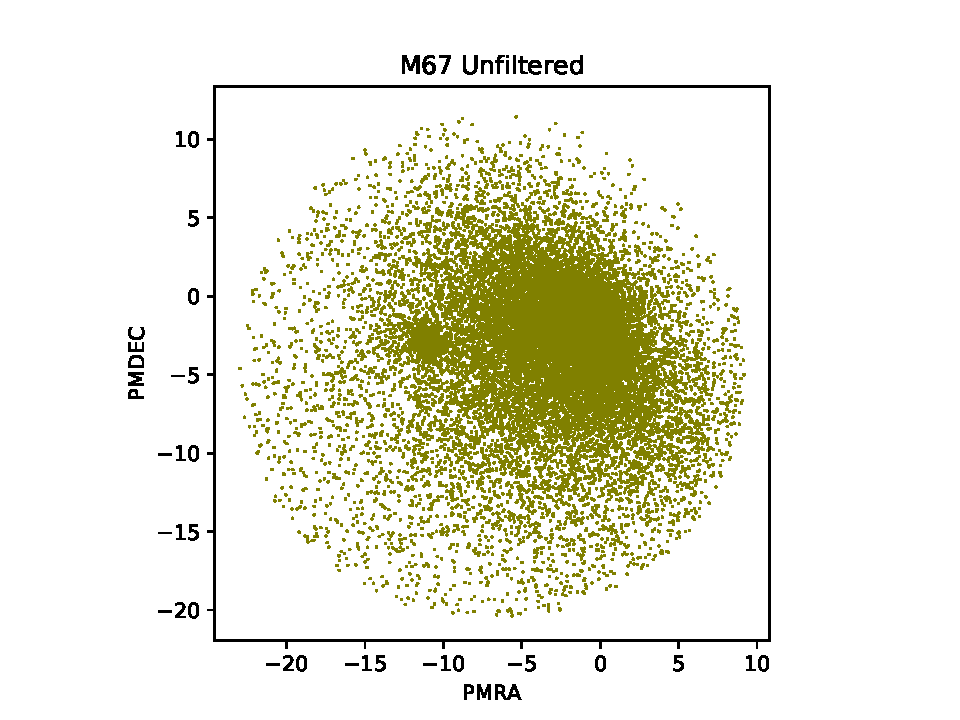
\includegraphics[width=4in]{M67_pm_unfiltered.pdf}
	\caption{Plot of the proper motion in the DEC versus proper motion in the RA for M67. The tight clumping left of center is the region that is selected when filtering. Stars outside of this region are considered contamination}
	\label{fig:M67_pos}
\end{figure}


\begin{figure}[!h]
	\centering
      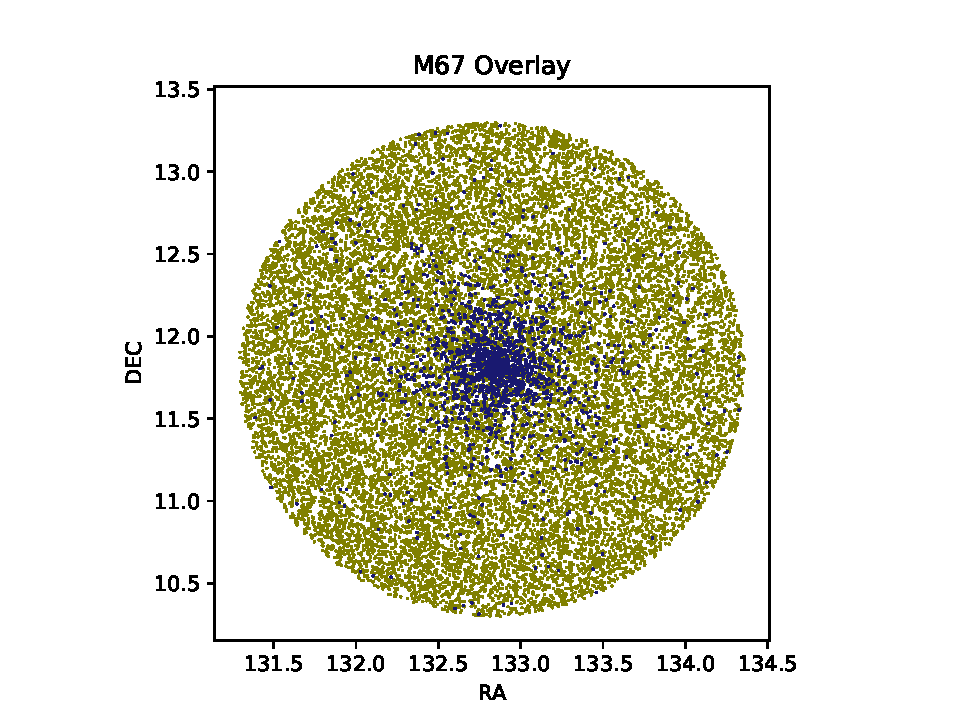
\includegraphics[width=4in]{M67_ra_dec_overlay.pdf}
	\caption{Plot of the declination versus the right ascension for a 1.5 degree radius around M67. Blue points represent members of the cluster post-filtering, and green points represent stars that have been filtered out.}
	\label{fig:M67_pos}
\end{figure}

Often the proper motion filtering is not enough though. Theoretically, filtering by radial velocity in addition to proper motion would help to effectively remove a vast majority of the remaining stars that do not belong to the cluster. However, because stars in a cluster are generally in close proximity, Gaia does not have uncontaminated radial velocity measurements for a vast majority of the stars in the field. My solution in reducing a majority of the noise from a simple proper motion filtering technique is to use a multi-phase approach. First, I create a temporary truncated data set of stars whose brightness is above a certain threshold. The reason for this is that typically the stars that I don't care about are farther away than the cluster and therefore quite dim in apparent brightness. I then filter the bright stars by proper motion and calculate the mean parallax. From here, I then filter the original data set by the mean parallax and then again by the proper motion, giving a data set that includes the dim stars but greatly reduces background and foreground contamination compared to the naive approach. This method typically reduces an unfiltered data set of 20-50 thousand stars down to a few thousand stars. The improvements of this fitting technique can be seen in the comparison of Figures \ref{fig:M67_CMD_filtered} \& \ref{fig:MS_spread}. Figure \ref{fig:MS_spread} makes use of the enhanced filtering, which reduces the contamination around the main sequence seen in Figure \ref{fig:M67_CMD_filtered}. After filtering, I treat the remaining stars as members of the stellar cluster.

\section*{Color Magnitude Diagrams}
A valid question to have at this point is ``How do I know whether my filtering method is effective?''; this is where color magnitude diagrams come in. One of the main features of a CMD is the main sequence. The main sequence is a generally linear region of the diagram where stars `live' for a majority of their lifetime. This is to say that when plotting measured values of apparent magnitude and color index, properties which change depending on the composition and age of the star, the data point will generally end up on the main sequence for most of a star's lifetime. At one end of the main sequence is the main sequence turnoff. This feature of the diagram usually appears to curl back over the main sequence, and represents data points for stars that are in the late stages of their lives, typically undergoing a drastic change in internal fusion dynamics. 

Stars with different properties will appear on different tracks of the main sequence, or even a different main sequence altogether. However, we can still construct a real life CMD by plotting a group of stars that formed at roughly the same time and with the same chemical makeup. Generally, higher mass stars will evolve and die off more quickly. Because of this, even if the less massive stars have not had time to evolve up and off of the main sequence, there will still be stars that are present in our measurements to map out the majority of the main sequence and main sequence turnoff. What this means is that we can use how well the main sequence and turnoff are preserved as a proxy for how good of a filter we have.

Plotting a CMD for the unfiltered data along a given line of sight produces an unintelligible blob of data points, as seen in Figure \ref{fig:M67_CMD_unfiltered}. This is because stars in this region formed at widely different times and from different concentrations of elements. Stars without the same composition will not align to the same main sequence. After applying the previously discussed filtering techniques, a clear main sequence and turnoff become apparent, as seen in Figure \ref{fig:M67_CMD_filtered}. This not only helps to gauge filtering methods, but also demonstrates clearly that a formation of similar stars, a stellar cluster, exists in the line of sight. All determinations I have made in the effectiveness of various filtering techniques have come from meaningful differences in the post-filtering CMD. Though filtering by these parameters is effective, a fine balance needs to be maintained between filtering out non-members and erroneously filtering out members.

\begin{figure}[!h]
	\centering
      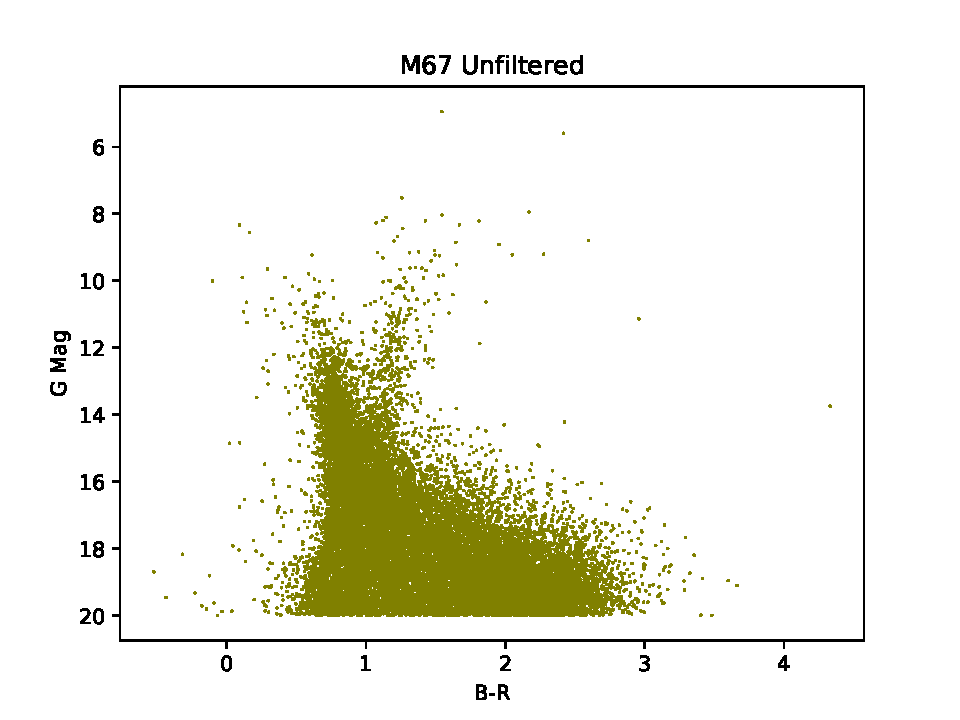
\includegraphics[width=3.5in]{M67_CMD_unfiltered.pdf}
	\caption{Color-Magnitude diagram of stars in M67 generated using unfiltered data from Gaia DR2.}
	\label{fig:M67_CMD_unfiltered}
\end{figure}

\begin{figure}[!h]
	\centering
      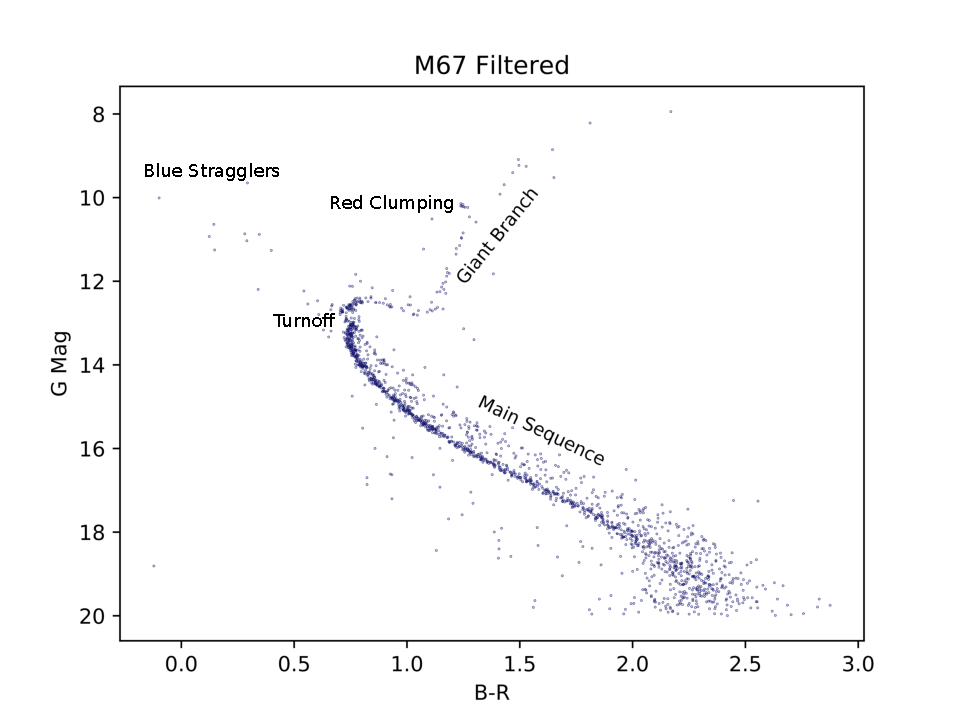
\includegraphics[width=3.5in]{M67_CMD_filtered.pdf}
	\caption{Color-Magnitude diagram of stars in M67 generated using filtered data from Gaia DR2. Many of the supplementary features mentioned are present on the plot, including a secondary main sequence, red clumping, and blue stragglers.}
	\label{fig:M67_CMD_filtered}
\end{figure}

Visible on the the CMD for the cluster M67, as seen is Figure \ref{fig:M67_CMD_filtered}, are a few additional features. A less dense string of stars, called blue stragglers, appears to continue the main sequence trend line past the main sequence turnoff point. The exact origin of these blue stragglers is not known, but the most plausible explanation is that these stars formed later than the majority of the stars in the cluster. It is also possible that these blue stragglers are the result of stellar collisions. Another feature visible on the CMD for M67 is a phenomenon known as red clumping. In contrast to the relatively sparse data points past the main sequence turnoff point, there is a dense clumping of data points at one particular segment of the post-turnoff region. The reason for this clumping is that when lower mass stars are evolving off of the main sequence, their hydrogen core has fused into a core of helium. Stars build up a core of helium until a point where the conditions are right for helium fusion to spontaneously begin, known as a helium flash. Stars tend to spend a longer time in the helium fusing stage compared to other stages past the main sequence, causing a higher density of points on the CMD relative to the other stages past the turnoff.

Also of note on the CMD for M67 when compared to a theoretical main sequence, is that the main sequence has a spread to it. The dimmer edge of the main sequence is relatively well defined and dense. Conversely, the the brighter edge of the main sequence line is less well defined and the space above the dimmer edge is considerably less data point dense. I believe the reason for this phenomenon is due to the presence of binary stars. Binary stars are a system of two stars that are orbiting close to each other, and are therefore often observed as a single point source star. If two stars orbiting each other had roughly the same color index and magnitude, then when they are observed side by side relative to the line of sight, they would appear twice as bright as a single star with the same color index on the main sequence. As the stars orbit, they would reach a minimum brightness of that of a single star of that color index, with one star behind the other. Any combination of stars between these two states, with partial eclipsing, or stars of unequal color or magnitude, would produce the spread of points seen between these two edges. Therefore, I believe that the more dense bottom edge is made up of single and eclipsing binary stars, while the upper edge and the spread between is comprised of binary stars that are uneclipsed or partially eclipsing. In order to confirm this, I fit two lines to a segment of the main sequence with identical slope, one line to each edge of the main sequence. Magnitude is logarithmic, so a doubling in brightness would correspond to a 0.75 magnitude shift as seen by the formula $m_1-m_2 = -2.5\text{log}\left(\frac{I_1}{I_2}\right)$. I found that the lower and upper edges of the main sequence to be between 0.7 and 0.8 magnitudes apart, helping to solidify the theory about binary stars. A demonstration of this can be seen in Figure \ref{fig:MS_spread}.


\begin{figure}[!h]
	\centering
      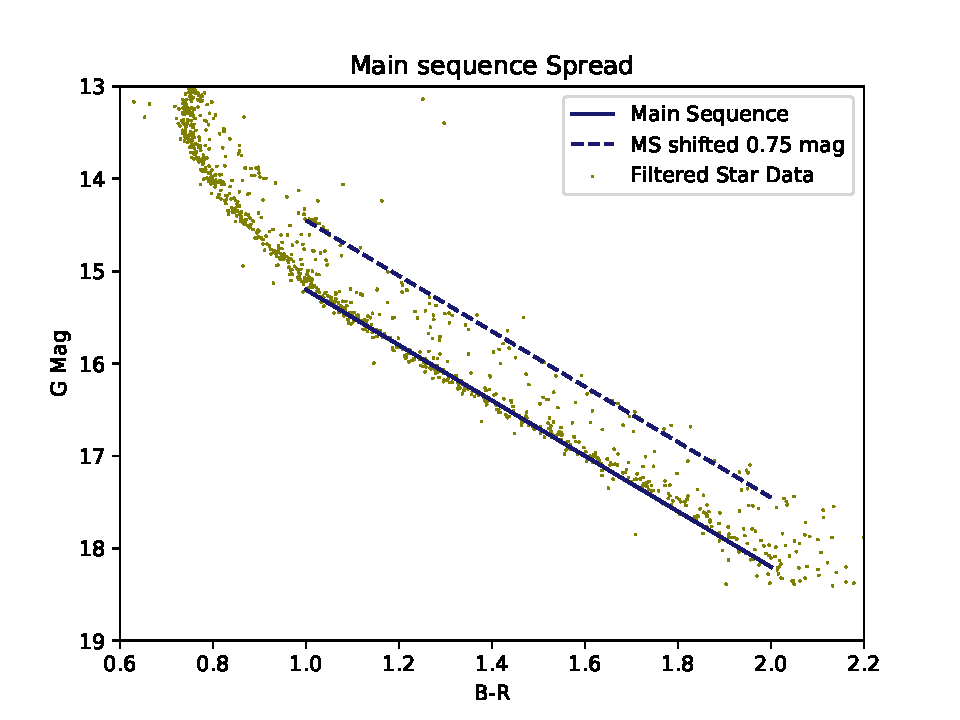
\includegraphics[width=3.5in]{M67_MS_Spread.pdf}
	\caption{Color-Magnitude diagram showing the spread in main sequence stars and the 0.75 magnitude separation between boundaries.}
	\label{fig:MS_spread}
\end{figure}


\section*{Isochrones}
Once I have a reasonably robust list of stellar cluster members, I can then determine some parameters about the cluster. I mentioned before that the age and composition of a group of stars needs to be similar in order for the main sequence to take shape. Because of this, we can infer properties about the age and composition of the cluster, whose members construct a connected main sequence. In astronomy, metallicity is a measure of the ratio of certain elements compared to the hydrogen and helium in a star. Metallicity is an important factor in studying larger scale stellar population evolution, because an older population of stars tends to have a lower metallicity than a younger population of stars. Measuring the age of the cluster also helps to confirm this relationship and further constrains stellar population evolution models.

By now, astronomers have a pretty good model for how typical stars evolve throughout their lifetime. Samples of model star data with a given age and metallicity are used to produce theoretical CMDs called isochrones. By comparing a series of isochrones to the cluster data and determining the goodness of fit, I am able to infer the age and metallicity of the cluster. A sample of a few different isochrones can be seen in Figure \ref{fig:Isochrone_Sample_Age} and Figure \ref{fig:Isochrone_Sample_Metallicity}. It is important to note that changes in metallicity tend to shift the isochrone horizontally, and changes in age shift the turnoff point further down the main sequence, towards the dimmer and redder stars. A further complication, however, is that interstellar reddening shifts the isochrone horizontally, and extinction shifts the isochrone vertically. Reddening and extinction are coupled proportionally, but without spectra to determine what color the star should be compared to its measured color index, it is difficult to properly identify the reddening. An example of the effect that reddening has on a cluster can be seen in Figure \ref{fig:reddening}.

\begin{figure}[!h]
	\centering
      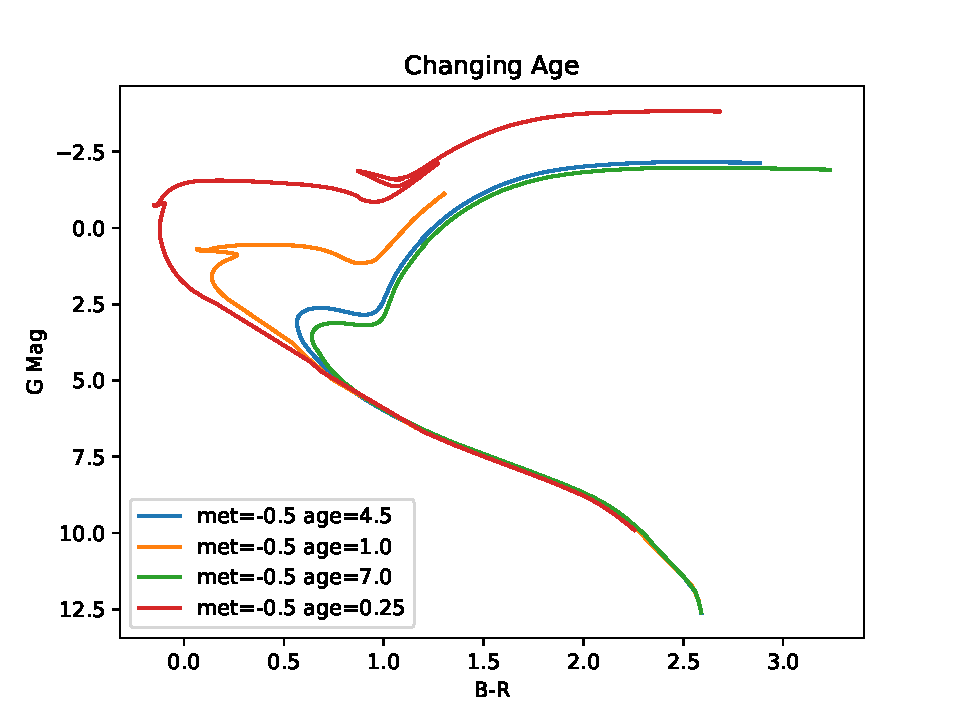
\includegraphics[width=3.5in]{iso_sample_age.pdf}
	\caption{Color-Magnitude diagram of various isochrones with a spread of ages in billions of years and the same metallicity.}
	\label{fig:Isochrone_Sample_Age}
\end{figure}

\begin{figure}[!h]
	\centering
      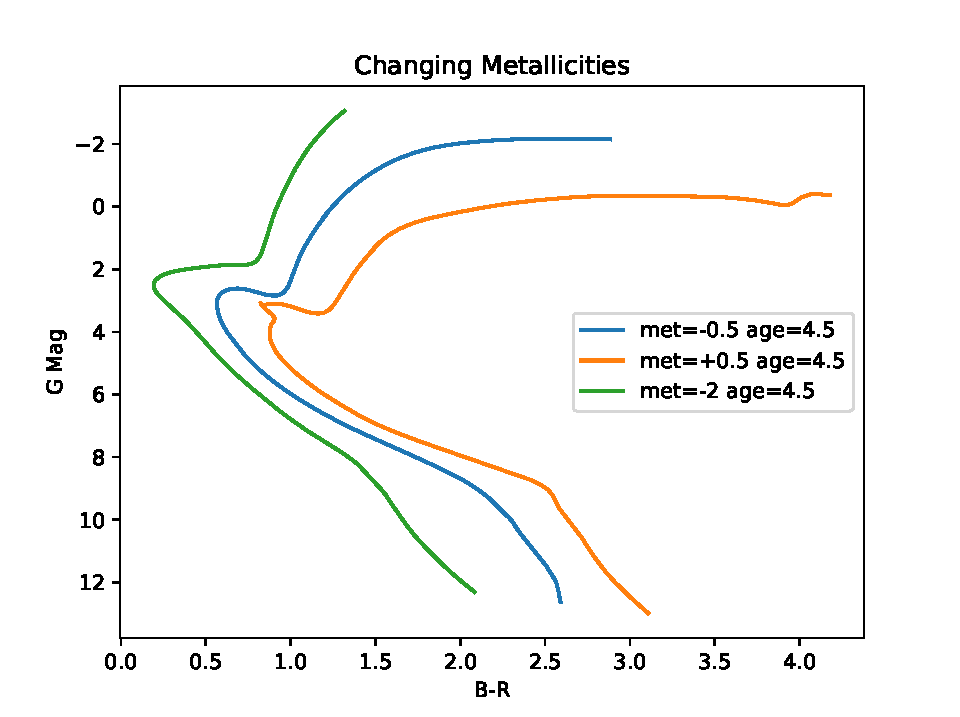
\includegraphics[width=3.5in]{iso_sample_metallicity.pdf}
	\caption{Color-Magnitude diagram of various isochrones with a spread of $\frac{Fe}{H}$ metallicities and the same age.}
	\label{fig:Isochrone_Sample_Metallicity}
\end{figure}

\begin{figure}[!h]
	\centering
      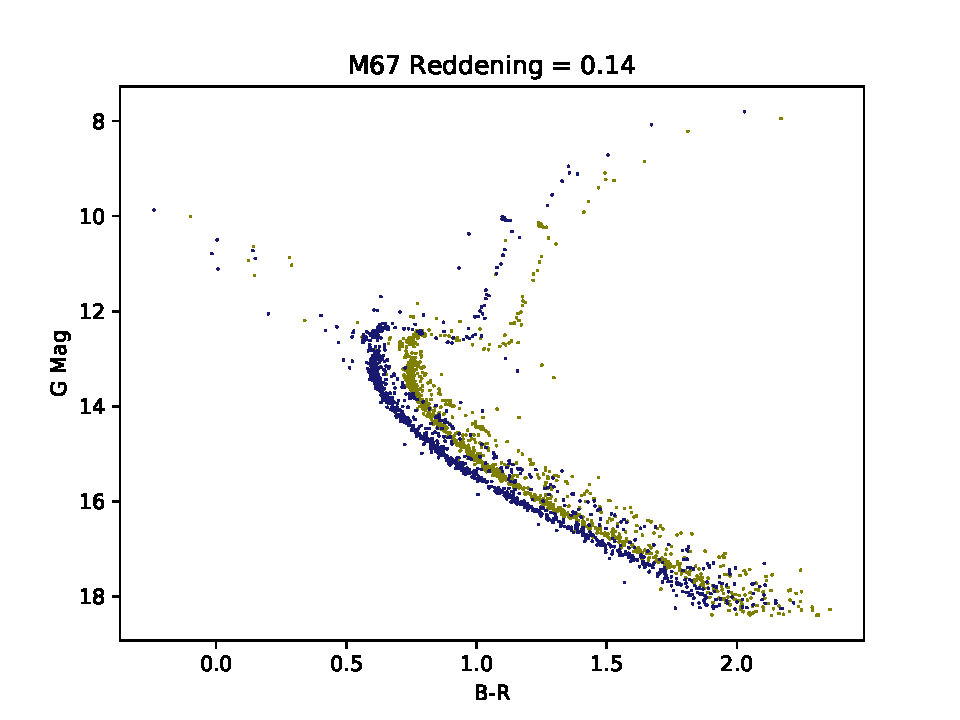
\includegraphics[width=3.5in]{reddening.pdf}
	\caption{Color-Magnitude diagram of M67 showing the ffects of reddening. The olive points represent the original data, and the blue points represent how M67 would look without the effects of reddening. Many clusters have an even more drastic change than this, and therefore it is a variable that needs to be controlled.}
	\label{fig:reddening}
\end{figure}

\section*{Fitting}
To fit the data from the clusters I have processed, I used isochrones provided by Dartmouth University's Stellar Evolution Database\protect{\cite{Isochrones}}. The isochrones are provided in steps of 250 million years, with a spread of values for metallicity in terms of both $\frac{Fe}{H}$ and $\frac{\alpha}{Fe}$. In other words, the fraction of iron to hydrogen, and of ``alpha'' to iron. Alpha in this case includes elements fused from helium nuclei, such as oxygen and silicon.

I have tried a few different methods of determining the best fit between the isochrone and the cluster data. The obvious, brute force method is to calculate the distance between every star and the isochrone and try to minimize the mean of these distance. Two issues arise with this approach. The first issue is that, depending on the number of stars left after filtering, the computational time required to determine this value is long. If your goal is to test several thousand isochrones to determine the best fit, then the computational time is prohibitively long. The other issue with this method is that there are a lot more points in the main sequence than past the main sequence. As a result, this method means you are selecting for isochrones that most closely match the main sequence, even at the cost of missing the post turnoff stars completely.

In order to account for the issues in statistical weight of the post main sequence turnoff stars, as well as the computational overhead, I condensed the data set into a spatially representative but statistically unrepresentative set of points. I segmented the CMD into vertically stacked slices, and took the median color index and magnitude in those bins to be a single point. The result of this is that a span of one magnitude in the main sequence is made up of roughly the same number of points as a one magnitude span post main sequence, which can be seen in Figure \ref{fig:weight}. This condensing of points serves to reduce the computational time drastically as well as to weigh the importance of the turnoff fit equally with the main sequence fit.

With the points condensed, I first attempted to fit the best isochrone by attempting to minimize the value:
\beq
\frac{1}{N}\sum\limits_{n=1}^{N}\sqrt{\left(x_n-x_{iso}\right)^2+\left(y_n-y_{iso}\right)^2}
\eeq
where $x_n$ and $y_n$ are a given condensed point's color index and G-band magnitude, $x_{iso}$ and $y_{iso}$ are the coordinates of the closest isochrone point, and $N$ is the total number of stars. In other words, I wanted to minimize the mean distance between the condensed points and their closest isochrone points.

I originally chose M67 because it is believed to have a reddening that is fairly negligible compared to other clusters. As a result, I could focus on fitting the isochrones to M67 without having to account for reddening. When it comes to other clusters, however, the reddening can impact the fit drastically, leaving me with three options. I could cite literature and hard code values for the reddening in for a given cluster, read in reddening information from Gaia, or process only clusters with known, negligible reddening. The Gaia measurements for reddening are sparse and seemingly inaccurate, so that left me with two choices. I chose to do none of these options, and instead sequentially determined the best fit for a whole series of reddening values. While the plausibility of fitting three parameters that each shift the position of the main sequence is dubious, the results have been extremely promising. I calculate the fit for each isochrone to a given cluster for every reddening from 0 to 1 in steps of 0.05, and weigh the fits of different reddening values against each other.

\section*{Other Clusters}

Much of my work throughout the second semester of capstone has been improving the filtering and fitting methods used to process M67. My aim in doing so has been to allow for a hands-off fitting of a wide variety of other clusters in order to test the robustness of these methods. While I have had the luxury of tailoring the fitting methods to work well for M67 for over a semester, the true test has been in determining the efficacy of those same methods when applied to different data sets. 

My second cluster that I have processed was Messier 35. M35 is quite drastically different to M67 in a few ways. While it is still an open cluster, it is quite considerably younger, meaning that the main sequence barely has a turn off point to be fit. This also proves as a limitation for how accurately the parameters can be determined, as the isochrones that I have been using only come in steps of 250 million years, which is the same order of magnitude as M35's accepted age. In contrast to M67, M35 also has quite pronounced reddening, which is likely due to the fact that it is much closer to the plane of the galaxy than our line of sight to M67 is. The extra interstellar dust in the way is what causes M35 to have a higher reddening. Given its positioning, the field of view around M35 is also host to a lot more stars, meaning reducing background and foreground contamination is also a greater challenge. With that said, the results of the filtering and fitting can be seen in Figure \ref{fig:M35_iso_best_fit}.

The next cluster I attempted to fit was NGC752. NGC is more similar to M67, with an expected age on the order of 2 billion years. While this is still on the low range for the set of isochrones available to me, it is a reasonably high age for open clusters. Clusters have a characteristic known as evaporation time, which is the timescale over which stars may be flung out of or stripped from the cluster due to gravitational interactions with the surrounding matter. Open clusters typically have a low evaporation time meaning that it is rare for them to last billions of years. I also tried to fit another cluster, NGC188, at the same time as NGC752. NGC 188 is extremely old, with an expected age of over 6.5 billion years. When fitting these clusters without any fine-tuning, the results were far from effective. For starters, one of the important steps in fitting the cluster is determining the turning point. This is done so that stars past the main sequence, i.e. blue stragglers, can be ignored. The location of the turnoff is also used to weigh the fit so that the turnoff is more important than the lower end of the main sequence. While the filtering methods worked well on these new clusters, the issues with fitting meant I had to further generalize the process.

\begin{figure}[!h]
	\centering
      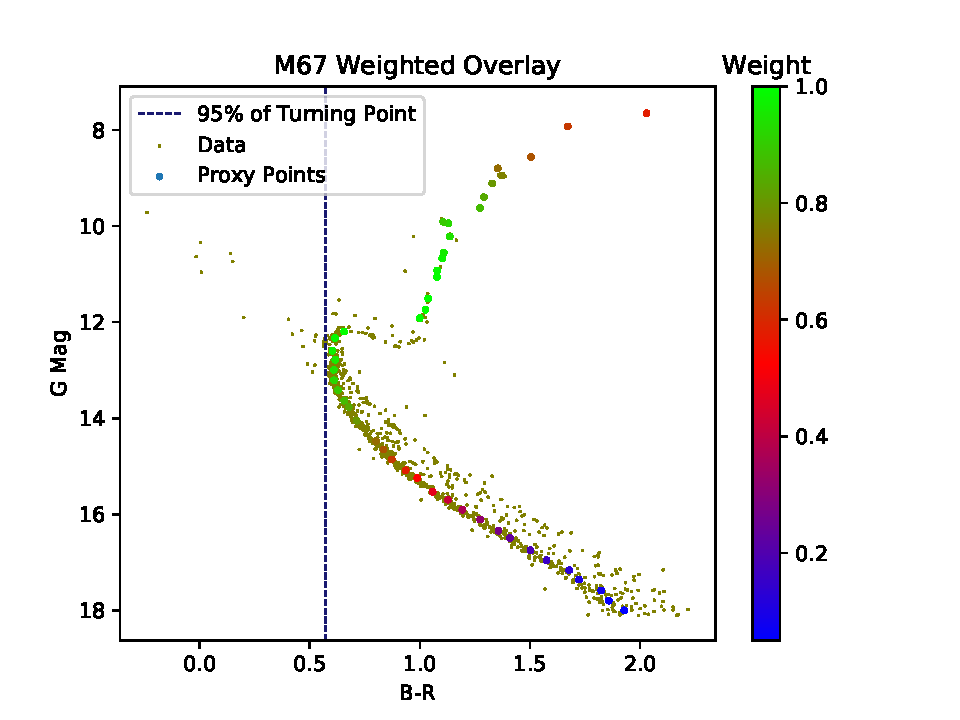
\includegraphics[width=3.5in]{weight.pdf}
	\caption{Example of a weight scheme shown on the plot for M67.Also seen is a vertical line just left of the determined turning point. Any data points left of this line, i.e. blue stragglers, have been ignored in the point condensing process.}
	\label{fig:weight}
\end{figure}

\section*{The Process Version 2.0}
The methods described above for filtering the data remains the same, concluding in a list of stars that are believed to be members of the cluster. Adjustments to the fitting method begin with the identification of the main sequence turnoff point. Previous methods involved looping through each condensed point, and determining the ratio of points to the left versus points to the right for all points above a given red point. While this worked for a cluster like M67, it did not work for a cluster like M35, whose post turnoff is poorly defined. My new method for finding the turnoff point is to fit a line to the first 12 or so condensed points, with the intention of these being those that make up the main sequence, and then fit a line from the lowest point to each point after the 12th. The angle between the 12 point baseline and every subsequent 2-point line is then assigned as a property to that point. The first point from bottom to top to cross a threshold angle $\theta_{crit}$ is determined to be the turning point. This method works remarkably well for M67, M35, and NGC188 with a default value of $\theta_{crit} = 5$. However, given the unusual shape of the main sequence of NGC752, the turnoff point determination is less successful.

Once the main sequence turnoff has been identified and the points re-condensed, each condensed point is assigned a weight based on its proximity to the turnoff point. Points past the turnoff also receive a higher weight than those on the main sequence. An example weighting can be seen in Figure \ref{fig:weight}. The condensed points are then fit against a series of over 73000 isochrones with varying ages, metallicities, and reddening values. In place of the previous method of minimizing the mean distance between each point, I now use a least-squares method. That is, I assign a score to each isochrone based on the sum of the distances between points, squared. Therefore, I am attempting to minimize the value:

\beq
\sum\limits_{n=1}^{N}\left[\left(x_n-x_{iso}\right)^2+\left(y_n-y_{iso}\right)^2\right]
\eeq

where again, $x_n$ and $y_n$ are a given condensed point's color index and G-band magnitude. $x_{iso}$ and $y_{iso}$ are the coordinates of the closest isochrone point. $N$, as always, represents the total number of stars for a given cluster. By minimizing this quantity instead of the mean distance, a few missed points are more likely to `throw out' an imperfect fit.

The trickiest part of fitting the newest clusters has been in adjusting the point weighing scheme. The results of the fit have proven very susceptible to minor changes in how the different condensed points are weighed. Moreover, a point weight scheme that works extremely well for one cluster may not work at all for another cluster. That is why, despite the time I have invested in determining point weight, I have created most of the plots without the use of any weight scheme for the purposes of this paper. The best identified fits for M67, M35, and NGC188 can be seen in Figures \ref{fig:M67_iso_best_fit}, \ref{fig:M35_iso_best_fit}, \& \ref{fig:NGC188_iso_best_fit} respectively. Some of the fits could be improved by searching the top 10 or 20 fits by eye, manually omitting a few points, or adjusting the weight parameters to individual clusters, but in this paper I'd like to highlight the outcome of my automated processing of these clusters without adulterating the results.

\begin{figure}[!h]
	\centering
      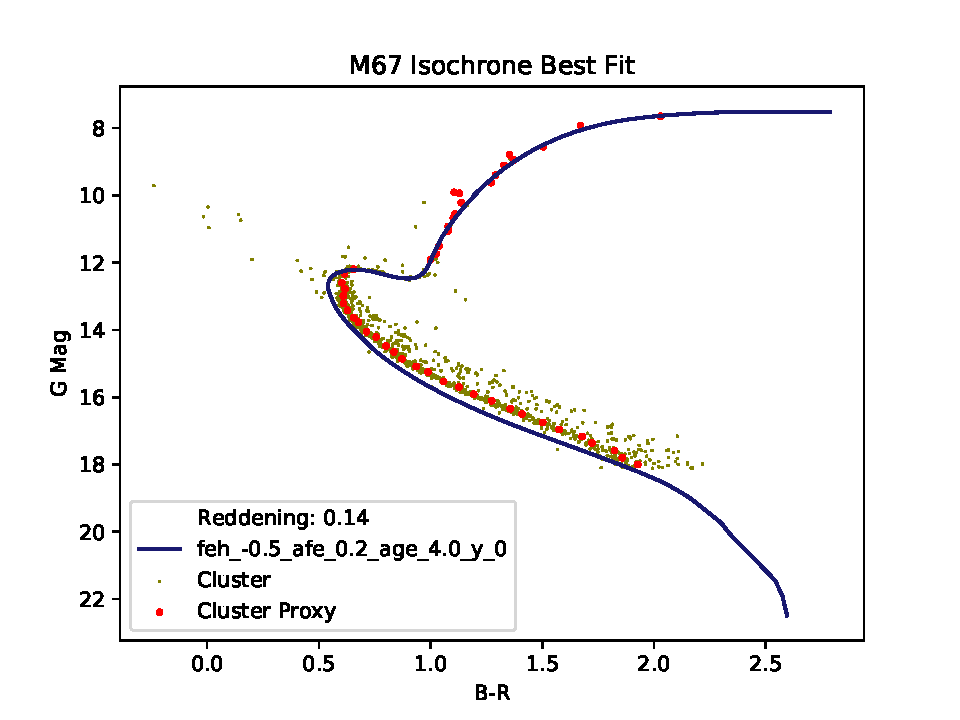
\includegraphics[width=3.5in]{M67_CMD_Iso_BestFit.pdf}
	\caption{Best fit determined for the cluster M67. Notable is that the main sequence is missed slightly by the best fit, but the turnoff and giant branch is fit very well. This leaves open to interpretation whether a better fit of the main sequence but a worse fit of the turnoff is more valid.}
	\label{fig:M67_iso_best_fit}
\end{figure}

\begin{figure}[!h]
	\centering
      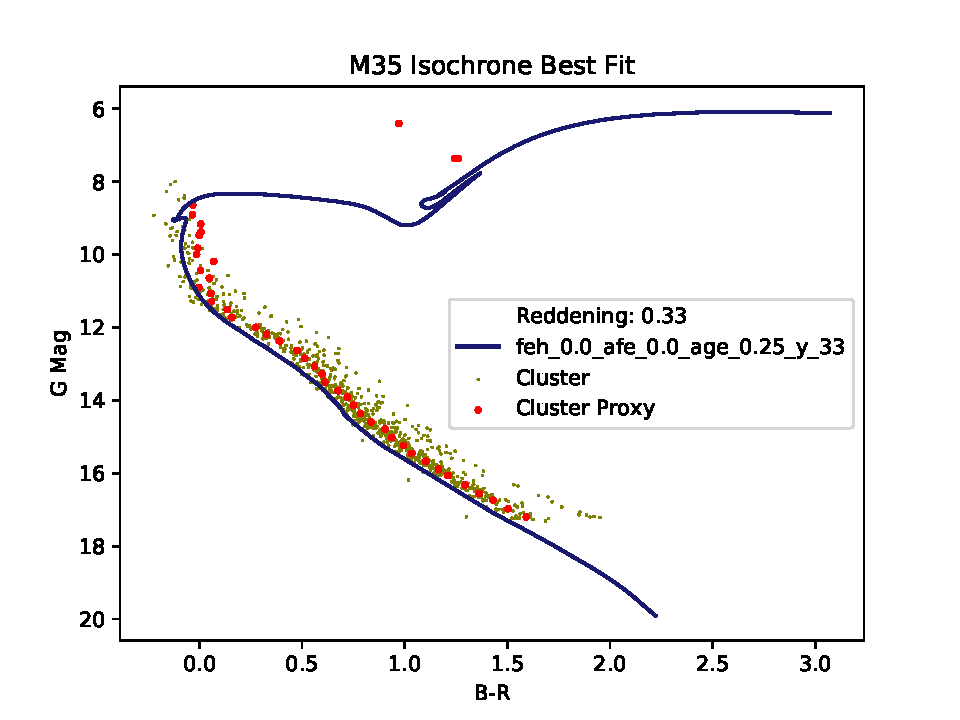
\includegraphics[width=3.5in]{M35_CMD_Iso_BestFit.pdf}
	\caption{Best fit determined for the cluster M35. Since the post-turnoff region is rather sparse on M35's CMD, the fit to the main sequence is more important. By eye, the shape of the main sequence of the isochrone is a good match to that of the CMD. There is likely a better fit for M35 were the points past the turnoff to be manually ignored.}
	\label{fig:M35_iso_best_fit}
\end{figure} 

\begin{figure}[!h]
	\centering
      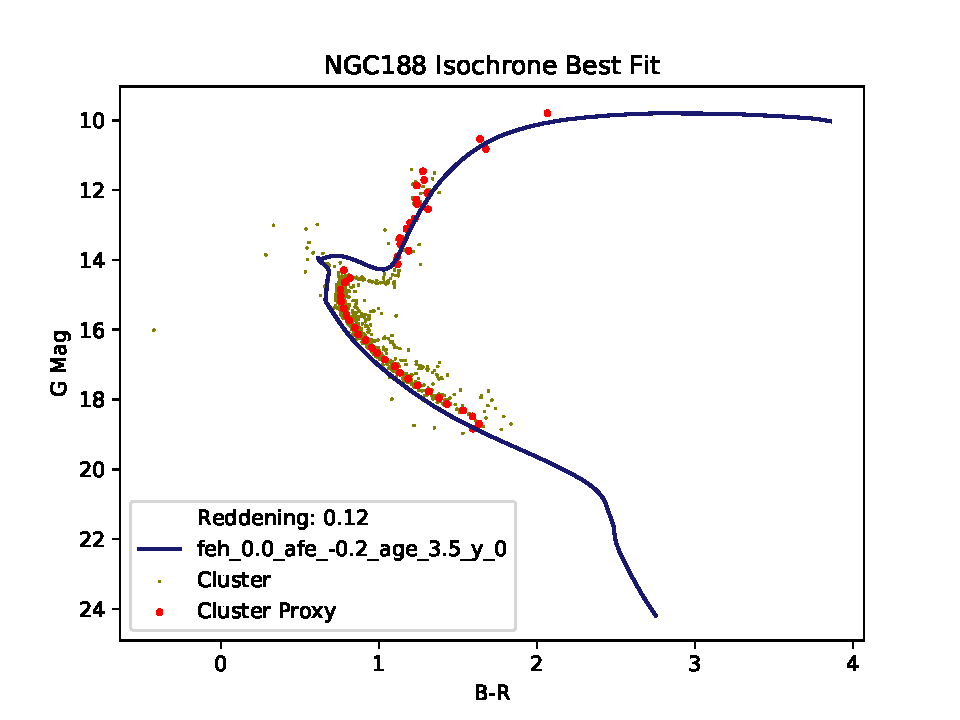
\includegraphics[width=3.5in]{NGC188_CMD_Iso_BestFit.pdf}
	\caption{Best fit determined for the cluster NGC188. The goodness of fit by eye is less agreeable than perhaps M67, but is generally close. As with all of the clusters, a better fit by eye often rests within the top ten scored fits, but for the purposes of the paper I have included my algorithm's selection as the best fit.}
	\label{fig:NGC188_iso_best_fit}
\end{figure}  

\section*{Uncertainties}
Measurements from the Gaia archive obviously come with uncertainties. While I have not included error bars on any of the fits that I have produced, I am able to give an upper limit on the uncertainty in the fit parameters for a few reasons. Firstly, the uncertainties in magnitude and color index scale with brightness. This means that fainter stars have higher uncertainties. Despite my improved filtering techniques, every cluster has some contamination in its CMD, especially at the fainter end. In order to make isochrone fitting smoother, I have clipped the main sequence off at a point there the uncertainties cross a set threshold. Where this clipping happens is dependent on the cluster, but is usually around 18 mag. Figure \ref{fig:gaiaTable} shows the relationship between uncertainties and G-band magnitude. You can see that from 17 to 20 the uncertainty increases by a factor of 7 in position and 6 in proper motion.

With stars having high uncertainties discarded, another thing to consider is the `resolution' of the parameter space that I am given in the isochrone set. For starters, the ages of the isochrones only increment in steps of 250 million years. While this is a lot of time compared to the human lifespan, it is quite a coarse step when looking at astronomical phenomena. There are dozens of nearby open clusters that I cannot effectively analyze via this project because they are all much younger than 250 million years. Even for older clusters, the step size in age for the isochrones limits how accurate of an assignment I can give. With this in mind, I assign an uncertainty equal to the step size of 0.25 Gyr of the fits for age.

The isochrones also have a limited spread in both $\frac{Fe}{H}$ and $\frac{\alpha}{Fe}$ metallicities. $\frac{Fe}{H}$ has possible values of $\left\{0,-0.5,-1.0,-1.5,-2.0,-2.5\right\}$, and $\frac{\alpha}{Fe}$ has values of $\left\{-0.2,0,0.2,0.4,0.6,0.8\right\}$. The difference in the goodness of fit when changing between these parameters is quite significant. As such, I am quite comfortable reporting that the uncertainty in the best fit parameters is 0.2 for $\frac{\alpha}{Fe}$ and 0.5 for $\frac{Fe}{H}$. Because no meaningful difference in fit can be determined on a scale smaller than these values, they serve as an upper bound for uncertainty. A small fraction of isochrones have a third metallicity value of $Y$, which is either 0,0.33, or 0.4. As such, the uncertainty in these values is hard to gauge.

As for the uncertainty in reddening, I have chosen to fit isochrones in steps of 0.01 $E(BP-RP)$. This step size was chosen to balance computational time with resolution, and because there is very little visual difference between fits with a smaller step size than 0.01. My program stores a list of best fits in order of their score, and as such there are several fits that are good by eye. Usually, the top 5 fits tend to share the same age and metallicity but vary slightly in reddening, so for that reason I consider the uncertainty to be on the order of 0.02 $E(BP-RP)$. The extinction of the light from the cluster is related to the reddening by the formula $A_G = k*E(BP-RP)$. For the purposes of my program, I used a conversion factor of $k=2.1$ to shift the brightness of the isochrones in accordance with each reddening value. That is to say that a shift of 0.01 in color index corresponds to a 0.021 mag shift in magnitude.

\begin{figure}[!h]
	\centering
      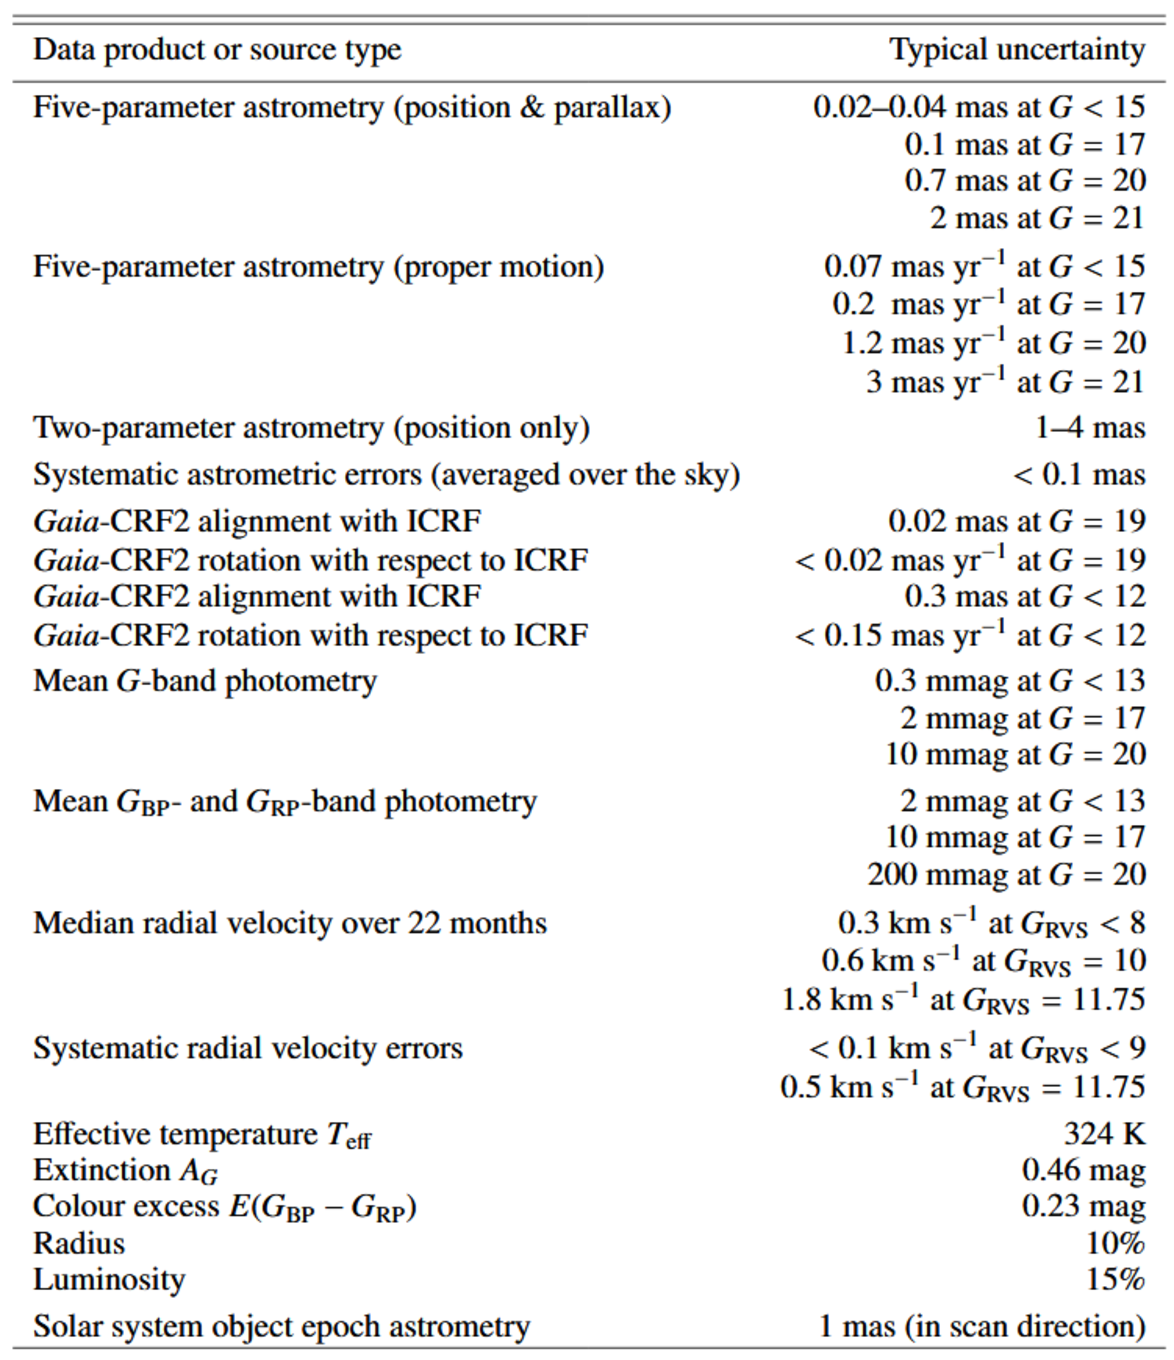
\includegraphics[width=3.5in]{gaiaTable.pdf}
	\caption{Basic performance statistics for Gaia DR2, taken from Gaia Collaboration et al.\protect{\cite{gaiaTable}}}
	\label{fig:gaiaTable}
\end{figure}


\section*{Conclusion}
As can be seen in Figures \ref{fig:M67_iso_best_fit}, \ref{fig:M35_iso_best_fit}, \& \ref{fig:NGC188_iso_best_fit}, the best fits as determined by the generic process work pretty well for a variety of cluster types. Unfortunately, a marginally better fit can often be determined by looking at the top 20 fits from the process output, and identifying the best fit by eye. That being said, in some cases, like that of M67, the best fit is the one identified by the algorithm. Given sufficient tweaking of the point weighting process, the fitting results could probably be more consistent across different data sets. The fit for NGC752 is a complete wash, because the automated detection of the turning point does not work correctly on this data set. This is something that could be addressed on a case by case basis, but therefore contradicts the point of a hands-off automated processing method. The parameters for the best fit can be seen in Table \ref{tab:results}. These values generally agree with the range of values reported as measurements in the SIMBAD\protect{\cite{simbad}} database. While most clusters have several measurements of $\left[\frac{Fe}{H}\right]$, I have been unable to find literature values for $\left[\frac{\alpha}{Fe}\right]$ to compare to.


\begin{table}[!h]
\begin{tabular}{|l|l|l|l|}
\hline
\textbf{Property}							& \textbf{M67}    & \textbf{M35}    & \textbf{NGC188}  \\ \hline
$\left[\frac{Fe}{H}\right]$      			& $-0.50\pm0.50$  & $+0.00\pm0.50$  & $+0.00\pm0.50$   \\ \hline
$\left[\frac{\alpha}{Fe}\right]$ 			& $+0.20\pm0.20$  & $+0.00\pm0.20$  & $-0.20\pm0.20$   \\ \hline
$E\left(BP-RP\right)$            			& $+0.14\pm0.02$  & $+0.33\pm0.02$ & $+0.12\pm0.02$    \\ \hline
Age (Gyr)                          			& $+4.00\pm0.25$  & $+0.25\pm0.25$  & $+3.50\pm0.25$   \\ \hline
$\left[Y\right]$                 			& $0$             & $0.33$          & $0$       \\ \specialrule{.2em}{.1em}{.1em}
$\left[\frac{Fe}{H}\right]$ Lit. & $-0.02\pm0.05$ & $-0.15$ & $-0.12\pm0.16$ \\ \hline
$E\left(BP-RP\right)$  Lit. & $+0.23\pm0.05$ & $+0.40$ & $+0.23\pm0.064$ \\ \hline
Age (Gyr) Lit. & $+3.85\pm0.17$ & $+0.15\pm0.05$ & $+7.70\pm1.40$ \\ \hline
\end{tabular}
\caption{\label{tab:results}Parameters with uncertainties from the best fits of each cluster, as determined by the automated process. The last three rows represent values from literature\protect{\cite{p1}\cite{p2}\cite{p3}\cite{p4}}. Literature values for $E\left(BP-RP\right)$  have been converted from $E\left(B-V\right)$.} 
\end{table}

Altogether, I am pleased with the outcome of this project, and I learned a lot about Python and Astronomy in the process. I hope to be able to apply the techniques and skills that I have learned during this project on my future endeavors, and wish that you, the reader, have learned something from my work.


\section*{Future Possibilities}
I am pleased with the extent of the project that I have been able to accomplish in my two semesters of capstone. While this likely is the end of this project for me, I still wish to conjecture about possible avenues of how my work could be applied. Most of what I would like to be able to accomplish were I given more time can be summarized as `doing science'. Were the algorithm sufficiently robust for varied types of clusters, then I could, for example, turn the algorithm loose on arbitrary patches of the sky to see if the code can find and characterize a cluster along that line of sight. This could potentially lead to the identification of unknown clusters, or just reaffirmation and further constraining of the age, metallicity, and reddening for known clusters. Another possibility is using the refined method of filtering to investigate cluster membership as a function of physical radius. This line of study would relate to topics like cluster evaporation and n-body dynamics. Regardless, I am glad to have been able to spend my last year at RIT exploring the stars.

\begin{acknowledgments}
I would like to thank my advisor, Dr. Richmond, as well as Dr. Bhattacharya, the capstone committee, and the RIT School of Physics and Astronomy.
\end{acknowledgments}
%
%change the name of the bibliography file to your own name
%make sure you have h-physrev5.bst file in the same directory as your tex file and bib file
%then compile using Latex-Bibtex-Latex-Latex sequence! <-- Quick Build, not Latex
%

\bibliographystyle{h-physrev5}
\bibliography{Wainwright_Capstone_II}

\end{document}

